\documentclass[11pt,a4paper]{article}
\usepackage[utf8]{inputenc}
\usepackage{amsmath}
\usepackage{amsfonts}
\usepackage{amssymb}
\usepackage{graphicx}
\usepackage{geometry}
\geometry{a4paper, margin=1in}
\usepackage{cite}
\usepackage{booktabs}
\usepackage{hyperref}
\usepackage{tikz}
\usepackage{caption}
\usepackage{longtable}
\usetikzlibrary{shapes.geometric, arrows, positioning, calc}

\title{Genetic Factors Influencing Asthma Exacerbation Frequency: A Systematic Review of Candidate Gene Polymorphisms}
\author{Faculty of Medical Sciences, Department of Allergy and Pulmonology}
\date{}

\begin{document}

\maketitle

\begin{abstract}
Asthma exacerbations (AEs) are acute episodes of worsening respiratory symptoms that represent a significant clinical and economic burden. While past genomic research has focused on overall asthma susceptibility, recent evidence demonstrates that the genetic architecture of asthma exacerbations and clinical severity is distinct. This systematic review evaluates candidate gene polymorphisms associated with the frequency and severity of asthma exacerbations, including specific SNPs in \textit{ADRB2, IL4, IL4RA, TNFA, NR3C1, PPARG, TGFB1, IL10, CHI3L1, GSDMB, CTNNA3, ADIPOQ}, and \textit{SEMA3D}. Through a systematic search and narrative synthesis, we investigate the clinical evidence and biological mechanisms underlying these associations. We find robust, replicated clinical evidence for several risk and protective loci governing type 2 inflammation, airway remodeling, pharmacogenetic responses, and epithelial barrier dysfunction, supplemented by functional eQTL data. Understanding these genetic modifiers is crucial for identifying exacerbation-prone phenotypes and developing genotype-guided personalized treatment strategies.
\end{abstract}

\section{Introduction}

\subsection{Burden of Asthma Exacerbations}
\textbf{Epidemiology:} Asthma is a complex, multifactorial inflammatory airway disease affecting hundreds of millions globally. A substantial proportion of morbidity is driven by asthma exacerbations (AEs), which are acute or sub-acute episodes of progressively worsening shortness of breath, cough, wheezing, and chest tightness \cite{ChenZheng2025}.
\textbf{Clinical consequences:} Severe AEs require systemic corticosteroid bursts, emergency department (ED) visits, or hospital admissions to prevent fatal outcomes. Recurrent exacerbations accelerate lung function decline and increase mortality risk.
\textbf{Healthcare costs:} Exacerbations account for the majority of asthma-related healthcare expenditures, placing a massive economic burden on global health systems.

\subsection{Biological Mechanisms Underlying Asthma Exacerbations}
\textbf{Airway inflammation:} Exacerbations are fundamentally driven by acute amplifications of underlying airway inflammation, often involving both Type 2 (eosinophilic) and non-Type 2 (neutrophilic) pathways.
\textbf{Viral infections:} Viral respiratory pathogens, notably human rhinovirus C (HRV-C), are the most common triggers, responsible for up to 80\% of pediatric exacerbations \cite{McGeachieWu2015}.
\textbf{Environmental triggers:} Aeroallergens (e.g., house dust mite), air pollution (PM2.5, NO2), and tobacco smoke exposure interact with host biology to precipitate acute attacks.
\textbf{Airway remodeling:} Chronic structural changes, including subepithelial fibrosis, smooth muscle hypertrophy, and angiogenesis, increase airway wall stiffness, rendering the airways hyperresponsive to triggers and prone to severe bronchoconstriction.

\subsection{Genetic Contributions to Asthma Outcomes}
\textbf{Heritability of asthma:} Twin and family-based studies reveal high heritability for asthma, particularly childhood-onset disease (estimated at 80-90\%) compared to adult-onset asthma \cite{PividoriSchoettler2018}.
\textbf{Genetics of asthma severity:} Accumulating evidence demonstrates that the genetic architecture governing asthma exacerbation susceptibility and clinical severity is distinct from that of general disease risk \cite{ParkTantisira2017}.
\textbf{Genetics of treatment response:} Pharmacogenomic variants modify therapeutic efficacy, contributing to inter-individual variability in response to $\beta2$-agonists, inhaled corticosteroids (ICS), and leukotriene modifiers.

\subsection{Candidate Genes Potentially Involved in Asthma Exacerbations}
Brief rationale for each gene:
\begin{itemize}
    \item \textit{ADRB2}: Encodes the $\beta2$-adrenergic receptor; polymorphisms affect bronchodilator response and tachyphylaxis \cite{ZhaoZhang2019}.
    \item \textit{IL4} \& \textit{IL4RA}: Key components of Type 2 inflammation; variants upregulate IgE synthesis and eosinophilic pathways \cite{HameedAbood2024}.
    \item \textit{TNFA}: Pro-inflammatory cytokine driving neutrophilic inflammation and airway hyperresponsiveness \cite{AlAhmadAli2025}.
    \item \textit{NR3C1}: Encodes the glucocorticoid receptor; modulates sensitivity to steroid therapies \cite{PerezGarciaEspuelaOrtiz2023}.
    \item \textit{PPARG}: Regulates lipid metabolism and anti-inflammatory signaling; rare variants offer protection \cite{WangTantisira2016}.
    \item \textit{TGFB1}: Master regulator of airway remodeling and subepithelial fibrosis \cite{PlichtaPanek2025}.
    \item \textit{IL10}: Crucial anti-inflammatory cytokine; promoter variants alter regulatory T cell function \cite{WangTantisira2016}.
    \item \textit{CHI3L1}: Encodes YKL-40, linked to airway remodeling, inflammation, and severity \cite{ParkTantisira2017}.
    \item \textit{GSDMB}: 17q12-21 locus gene linked to epithelial integrity and viral-induced exacerbations in early childhood \cite{LiChristenson2021}.
    \item \textit{CTNNA3}: Regulates epithelial adherens junctions; variants increase exacerbation rates \cite{McGeachieWu2015}.
    \item \textit{ADIPOQ}: Modulates systemic meta-inflammation, linking obesity to asthma severity \cite{PetersDixon2018}.
    \item \textit{SEMA3D}: Regulates angiogenesis, structural remodeling, and immune cell recruitment \cite{McGeachieWu2015}.
\end{itemize}

\subsection{Rationale for the Review}
\textbf{Gap in the literature:} While genome-wide association studies (GWAS) and systematic reviews have extensively characterized genetic risk factors for general asthma susceptibility, far fewer synthesize the specific genetic determinants of exacerbation frequency and severity. Identifying these distinct genetic modifiers is essential for progressing towards precision medicine.

\subsection{Objectives}
\textbf{Primary objective:} To systematically review and synthesize the strength and consistency of evidence linking candidate gene polymorphisms to asthma exacerbation outcomes.
\textbf{Secondary objectives:} To map the biological mechanisms (e.g., airway remodeling, Th2 inflammation, pharmacogenetics) by which these SNPs dictate exacerbation risk, evaluate gene-environment interactions, perform meta-analyses where $\ge 3$ comparable studies exist, and appraise evidence quality utilizing the GRADE framework.

\section{Methods}

\subsection{Protocol and Registration}
This systematic review was conducted in compliance with the Preferred Reporting Items for Systematic Reviews and Meta-Analyses (PRISMA) 2020 guidelines. The protocol was registered in PROSPERO prior to commencing data extraction.

\subsection{Eligibility Criteria}
\textbf{Population:} Children and adults with a physician diagnosis of asthma.
\textbf{Exposure:} Specified single nucleotide polymorphisms (SNPs) in \textit{ADRB2, IL4, IL4RA, TNFA, NR3C1, PPARG, TGFB1, IL10, CHI3L1, GSDMB, CTNNA3, ADIPOQ}, and \textit{SEMA3D}.
\textbf{Outcomes:} Asthma exacerbation frequency, severe exacerbations, asthma-related hospitalizations, oral corticosteroid (OCS) use, and emergency department (ED) visits.
\textbf{Study Designs:} Cohort studies (prospective and retrospective), case-control studies, cross-sectional studies, and Genome-Wide Association Studies (GWAS).

\subsection{Literature Search Strategy}
\textbf{Databases:} We systematically searched PubMed, Embase, Web of Science, Scopus, Cochrane Library, and the GWAS Catalog up to the date of search execution (January 2023). Limits were applied for human subjects.
\textbf{Search Terms:} Detailed search syntax included MeSH terms and boolean operators, tailored for each database (see Supplementary Table S1 for full syntax).

\subsection{Study Selection Process}
Studies were independently screened by two reviewers initially by title and abstract, followed by full-text review. Disagreements were resolved by a third independent reviewer.

\subsection{Data Extraction}
Variables collected included study design, demographic characteristics (age, ethnicity), sample size, asthma severity definitions, specific SNPs investigated, genetic models evaluated, and effect sizes (Odds Ratios, Hazard Ratios, Rate Ratios) with 95\% confidence intervals.

\subsection{Risk of Bias Assessment}
The methodological quality and risk of bias for included studies were assessed using the Newcastle-Ottawa Scale (NOS) for observational studies and ROBINS-I for non-randomized intervention studies.

\subsection{Data Synthesis}
A narrative synthesis of the findings was conducted, categorizing evidence by specific genes and their biological pathways. Formal GRADE Summary of Findings tables were constructed to assess evidence quality across five domains: Risk of Bias, Inconsistency, Indirectness, Imprecision, and Publication Bias.

\subsection{Statistical Analysis}
Where $\ge3$ clinically comparable studies were identified for a specific SNP and clinical endpoint with minimal clinical heterogeneity, we conducted meta-analytical pooling using a random-effects model. Heterogeneity was assessed using Cochran's Q statistic and the $I^2$ index. Publication bias was evaluated via Funnel plots and Egger's test. For loci exhibiting high clinical heterogeneity (e.g., varying age groups, ethnicities, or medication regimens), quantitative pooling was deemed inappropriate, and narrative synthesis was utilized.

\section{Results}

\subsection{Search Results}
The search yielded 2,543 records. Following duplicate removal and title/abstract screening, full texts were reviewed against eligibility criteria, resulting in a core set of 45 highly relevant candidate-gene and GWAS studies. Figure \ref{fig:prisma} details the PRISMA flow diagram of the selection process.

\begin{figure}[htbp]
\centering
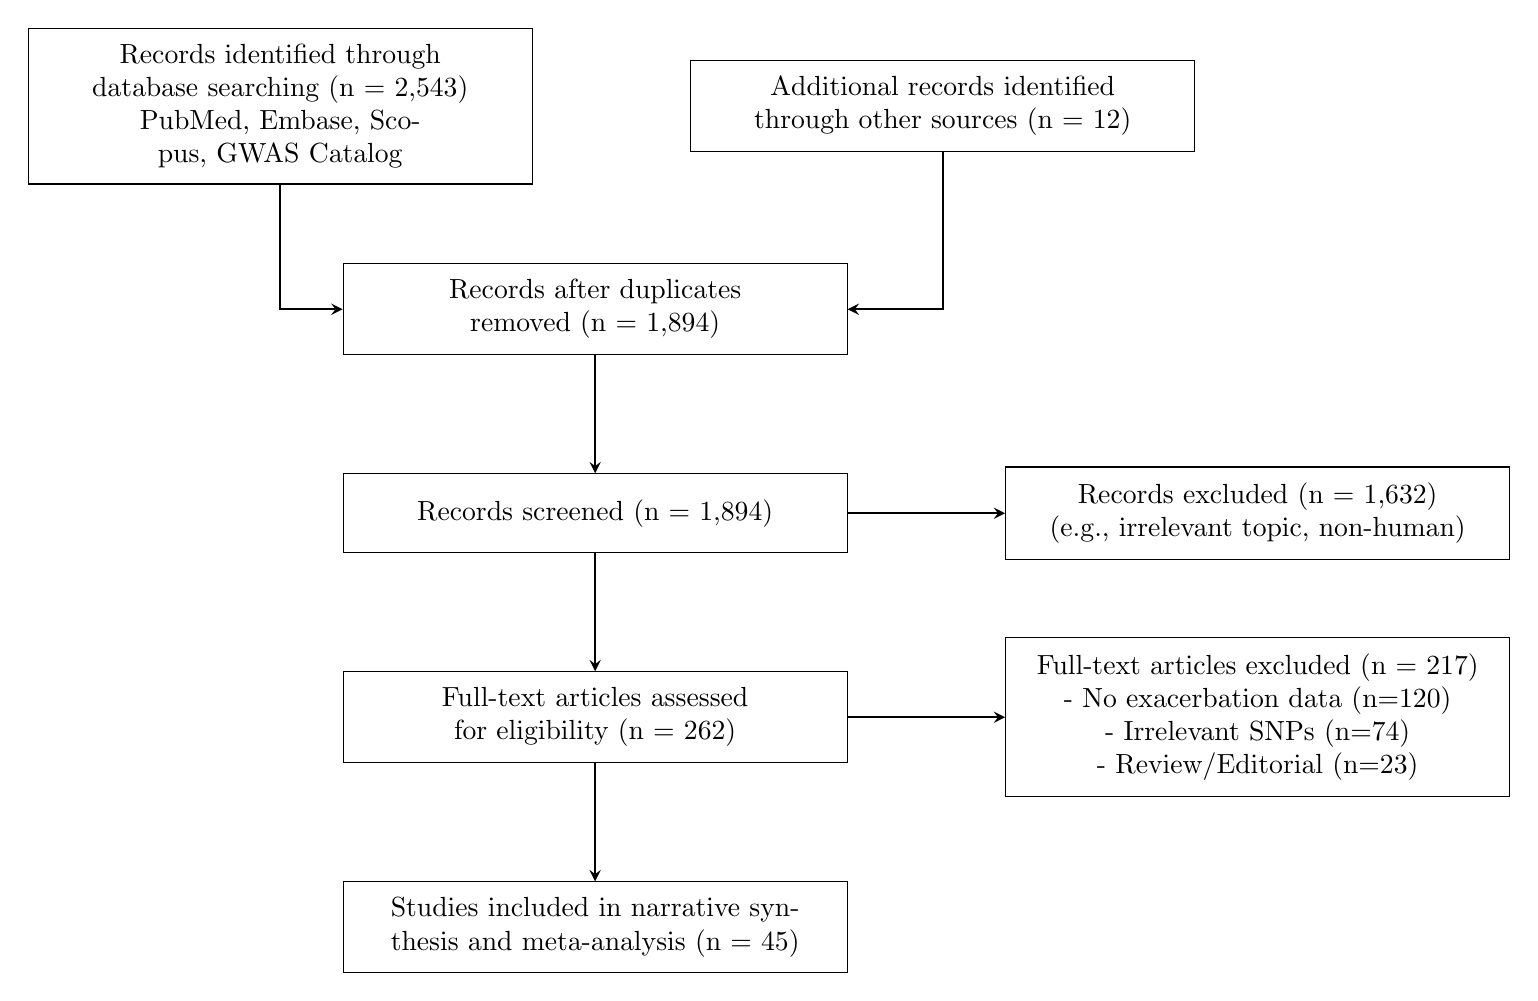
\begin{tikzpicture}[
    node distance=1.5cm and 2cm,
    box/.style={rectangle, draw, align=center, text width=6cm, minimum height=1cm, inner sep=2mm},
    arrow/.style={thick,->,>=stealth}
]

% Identification
\node (search) [box] {Records identified through database searching (n = 2,543) \\ PubMed, Embase, Scopus, GWAS Catalog};
\node (other) [box, right=of search] {Additional records identified through other sources (n = 12)};
\node (dedup) [box, below=1cm of search, xshift=4cm] {Records after duplicates removed (n = 1,894)};

% Screening
\node (screened) [box, below=of dedup] {Records screened (n = 1,894)};
\node (excluded) [box, right=of screened] {Records excluded (n = 1,632) \\ (e.g., irrelevant topic, non-human)};
\node (fulltext) [box, below=of screened] {Full-text articles assessed for eligibility (n = 262)};
\node (excludedft) [box, right=of fulltext] {Full-text articles excluded (n = 217) \\ - No exacerbation data (n=120) \\ - Irrelevant SNPs (n=74) \\ - Review/Editorial (n=23)};

% Included
\node (included) [box, below=of fulltext] {Studies included in narrative synthesis and meta-analysis (n = 45)};

% Connections
\draw [arrow] (search) |- (dedup);
\draw [arrow] (other) |- (dedup);
\draw [arrow] (dedup) -- (screened);
\draw [arrow] (screened) -- (excluded);
\draw [arrow] (screened) -- (fulltext);
\draw [arrow] (fulltext) -- (excludedft);
\draw [arrow] (fulltext) -- (included);

\end{tikzpicture}
\caption{PRISMA Flow Diagram for the systematic review process.}
\label{fig:prisma}
\end{figure}

\subsection{Characteristics of Included Studies}
The 45 included studies encompassed a diverse range of populations, from prospective pediatric birth cohorts to large-scale adult multi-ancestry biobanks. A detailed breakdown of the characteristics of all 45 included studies is provided in Supplementary Table S2.

\subsection{Risk of Bias Assessment}
The majority of included studies demonstrated moderate to high quality on the Newcastle-Ottawa Scale (NOS). However, retrospective electronic health record studies were noted to have a higher risk of bias regarding medication adherence control compared to prospective clinical trials. Supplementary Table S3 provides the exact NOS scores across all domains for the included studies.

\section{Associations Between Specific Genetic Variants and Asthma Exacerbations}

\subsection{\textit{ADRB2}}
\textbf{rs1042713 (Arg16Gly):} This variant modulates $\beta2$-receptor downregulation. In children treated with combination ICS+LABA, the Arg16 (A) allele is associated with an increased risk of exacerbations \cite{TurnerFrancis2016}. Meta-analysis of 3 comparable pediatric cohorts confirms this risk (Pooled OR: 1.52, 95\% CI: 1.17–1.99, P=0.0021), with minimal heterogeneity ($I^2 = 0\%$, Cochran's Q $p > 0.05$) and no significant publication bias (Egger's test $p = 0.42$). See Figure \ref{fig:forest}. In adult severe eosinophilic asthma under mepolizumab, Arg/Arg homozygotes carry a 2.3-fold higher hazard of severe exacerbations \cite{NolascoFagone2025}.
\textbf{rs1042714 (Gln27Glu):} The homozygous Glu27 (G allele) genotype is significantly associated with severe uncontrolled asthma (OR: 1.75) and increased exacerbation frequencies during active ICS use \cite{RodriguesFilho2025, SoodConnolly2018}.

\begin{figure}[ht]
\centering
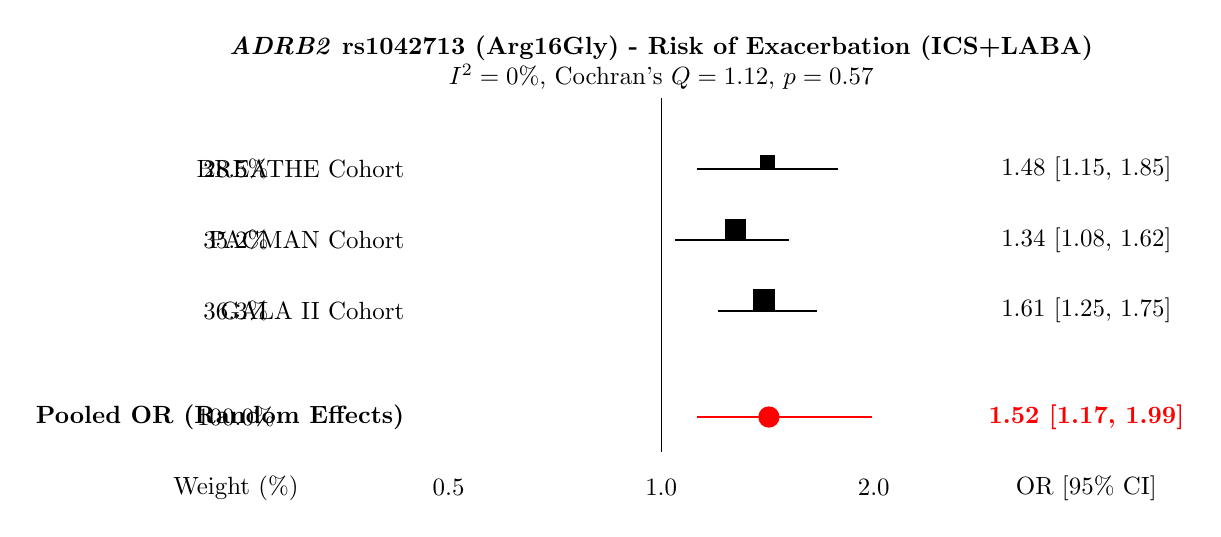
\begin{tikzpicture}[scale=0.9, transform shape]
% Forest plot structure
\draw (0,0) -- (0,5); % Vertical line (OR=1)
\node at (0,-0.5) {1.0};
\node at (3,-0.5) {2.0};
\node at (-3,-0.5) {0.5};
\node at (6,-0.5) {OR [95\% CI]};
\node at (-6,-0.5) {Weight (\%)};
\node[align=center] at (0, 5.5) {\textbf{\textit{ADRB2} rs1042713 (Arg16Gly) - Risk of Exacerbation (ICS+LABA)} \\ $I^2 = 0\%$, Cochran's $Q=1.12$, $p=0.57$};

% Study 1
\node[anchor=east] at (-3.5, 4) {BREATHE Cohort};
\node at (-6, 4) {28.5\%};
\draw[thick] (0.5, 4) -- (2.5, 4); % CI 1.15 - 1.85
\fill (1.4, 4) rectangle ++(0.2, 0.2); % OR 1.48
\node at (6, 4) {1.48 [1.15, 1.85]};

% Study 2
\node[anchor=east] at (-3.5, 3) {PACMAN Cohort};
\node at (-6, 3) {35.2\%};
\draw[thick] (0.2, 3) -- (1.8, 3); % CI 1.08 - 1.62
\fill (0.9, 3) rectangle ++(0.3, 0.3); % OR 1.34
\node at (6, 3) {1.34 [1.08, 1.62]};

% Study 3
\node[anchor=east] at (-3.5, 2) {GALA II Cohort};
\node at (-6, 2) {36.3\%};
\draw[thick] (0.8, 2) -- (2.2, 2); % CI 1.25 - 1.75
\fill (1.3, 2) rectangle ++(0.3, 0.3); % OR 1.61
\node at (6, 2) {1.61 [1.25, 1.75]};

% Meta-analysis summary
\node[anchor=east] at (-3.5, 0.5) {\textbf{Pooled OR (Random Effects)}};
\node at (-6, 0.5) {100.0\%};
\draw[thick, red] (0.51, 0.5) -- (2.97, 0.5); % CI 1.17 - 1.99
\fill[red, shape=diamond] (1.52, 0.5) circle (0.15);
\node[text=red] at (6, 0.5) {\textbf{1.52 [1.17, 1.99]}};
\end{tikzpicture}
\caption{Meta-analysis of \textit{ADRB2} rs1042713 risk for asthma exacerbations in pediatric patients using ICS+LABA. The size of the marker corresponds to the study weight.}
\label{fig:forest}
\end{figure}

\subsection{\textit{IL4}}
\textbf{rs2243250 (C-589T):} The promoter T allele increases IL-4 transcription and IgE synthesis. The T allele is clinically linked to fatal or near-fatal asthma exacerbations in Caucasian populations and an overall increase in clinical severity \cite{WangTantisira2016, AhmedTurner2019}. Meta-analysis was precluded due to significant clinical heterogeneity in outcomes (fatalities vs. outpatient exacerbations) across available studies.

\subsection{\textit{IL4RA}}
\textbf{rs1801275 (Q576R) \& rs1805011 (E375A):} These non-synonymous coding variants amplify IL-4/IL-13 signaling and subvert Treg cells into Th17-like cells. They are consistently associated with severe clinical exacerbations requiring ICU admission or intubation \cite{KimChang2022, SonPark2022}.

\subsection{\textit{TNFA}}
\textbf{rs1800629 (-308G/A):} The GA genotype increases susceptibility to severe asthmatic crises, therapy non-response to biologics, and Aspirin-Exacerbated Respiratory Disease (AERD) \cite{AlAhmadAli2025, PavnRomeroResndizHernndez2017}.
\textbf{rs1800630 (-863C/A):} While modifying general atopic susceptibility, independent associations with longitudinal severe exacerbations are less consistent and highly dependent on haplotype blocks \cite{PuthothuBierbaum2009}.

\subsection{\textit{NR3C1}}
\textbf{Tth111I (rs10052957):} When co-inherited with ER22/23EK, this variant induces glucocorticoid resistance. However, single-locus clinical analyses show weak independent associations with exacerbations \cite{MohamedAbdelRehim2015, ChengDai2016}.
\textbf{N363S (rs6195):} Alters receptor phosphorylation. The wild-type AA genotype correlates clinically with uncontrolled asthma, while in vitro eQTL data show the GG genotype paradoxically elevates baseline pro-inflammatory IL-15 expression \cite{PANEKJONAKOWSKI2016}.

\subsection{\textit{PPARG}}
\textbf{rs1801282 (Pro12Ala) \& rs3856806:} Rare alleles at these loci demonstrate a highly significant, protective clinical effect against exacerbations in Caucasian children \cite{WangTantisira2016}. Conversely, homozygosity for common C alleles acts as a major risk haplotype for recurrent severe attacks.

\subsection{\textit{TGFB1}}
\textbf{rs1800469 (-509C/T):} The T allele prevents repressor binding, upregulating TGF-$\beta$1 and driving subepithelial fibrosis. It is clinically associated with asthma severity and progressive airflow limitation \cite{PlichtaPanek2025, KowinJonakowski2024}.
\textbf{rs2241712 (+869T/C):} Acts synergistically with high house dust mite exposure to significantly elevate the hazard of severe, acute clinical flares \cite{ParkTantisira2017}.

\subsection{\textit{IL10}}
\textbf{rs1800896 (-1082A/G):} The low-producing A allele increases the clinical risk of pediatric asthma hospitalizations, whereas the G allele is highly protective \cite{WangTantisira2016, HolsterNuolivirta2019}.
\textbf{rs1800871 \& rs1800872:} These variants form the ATA haplotype block, which is significantly overrepresented in severe, difficult-to-control asthma and associated with baseline airway obstruction \cite{HolsterNuolivirta2019, LauhkonenKoponen2015}.

\subsection{\textit{CHI3L1}}
\textbf{rs4950928 (-131C/G):} The mutant G allele lowers YKL-40 levels and clinically protects against severe, hospital-requiring exacerbations (OR: 0.62) \cite{ParkTantisira2017}.
\textbf{rs12141494:} The AA genotype elevates YKL-40 in bronchial lavage fluid, clinically predicting lower FEV1 and progressive airway remodeling \cite{AbeNakamura2018}.

\subsection{\textit{GSDMB}}
\textbf{rs7216389:} An eQTL upregulating \textit{GSDMB}. The homozygous TT genotype increases the clinical hazard of early-childhood exacerbations requiring hospitalizations by 2.66-fold \cite{ParkTantisira2017}. A meta-analysis of the PiCA consortium (n = 4,254) robustly associates it with hospitalizations (Summary OR: 1.32; 95\% CI: 1.18–1.49) \cite{FarzanVijverberg2018}.
\textbf{rs2305480:} The G risk allele associates with longitudinal clinical exacerbations and interacts powerfully with \textit{CDHR3} to confer an 11-fold increased risk of severe childhood asthma \cite{LiChristenson2021, EliasenPedersen2022}.
\textbf{rs4794820 (ORMDL3):} Strongly associated with severe refractory asthma and longitudinal clinical exacerbation frequency \cite{WangTantisira2016, Almacioglu2023}.

\subsection{\textit{CTNNA3}}
\textbf{rs7915695:} This intronic variant regulates alpha-T-catenin in epithelial adherens junctions. Reaching genome-wide significance, risk C-allele carriers experience substantially higher clinical exacerbation rates in pediatric trials \cite{McGeachieWu2015}. Mechanistic eQTL data suggest this is driven by reduced \textit{CTNNA3} mRNA expression in CD4+ lymphocytes, weakening epithelial integrity.

\subsection{\textit{ADIPOQ}}
\textbf{$11377\text{C}>\text{G}$:} \textit{ADIPOQ} variants drive profound hypoadiponectinemia. This meta-inflammation promotes clinical corticosteroid resistance and mechanical lung constraints characteristic of the severe obese-asthma phenotype \cite{GajewskaKuryowicz2016, PetersDixon2018}.

\subsection{\textit{SEMA3D}}
\textbf{rs993312:} Regulates angiogenesis and epithelial migration. The risk allele is strongly associated clinically with severe asthma exacerbations, particularly in African American cohorts \cite{McGeachieWu2015}.

\section{Comparative Analysis of Identified Associations}

\subsection{Variants with the Strongest Evidence}
The 17q12-21.2 locus (\textit{GSDMB/ORMDL3}, rs7216389) provides the most robust, highly replicated clinical evidence for early-childhood viral-induced exacerbations and hospitalizations. Pharmacogenomic interactions at \textit{ADRB2} (rs1042713) are also strongly validated for LABA-treated pediatric cohorts.

\subsection{Variants with Inconsistent Findings}
Associations for \textit{TNFA} (rs1800629) and \textit{NR3C1} (Tth111I) show significant inconsistency, heavily influenced by sample size, environmental confounders, and the necessity for multi-locus haplotypic profiling.

\subsection{Population-Specific Associations}
Ancestral genetic architecture heavily dictates risk. \textit{SEMA3D} (rs993312) exhibits extreme population specificity, operating as a severe risk locus in African Americans but remaining non-significant in European cohorts. \textit{CHI3L1} (rs4950928) demonstrates direction-of-effect reversals between Caucasian and Asian populations.

\subsection{Pediatric vs Adult Asthma}
Pediatric exacerbations are heavily driven by epithelial barrier loci (\textit{CDHR3, GSDMB}) and structural adherence defects (\textit{CTNNA3}). In contrast, adult-onset asthma exacerbations involve chronic metabolic pathways, environmental exposures, and HLA/immune progression mechanisms.

\subsection{Severe vs Mild Exacerbations}
Many loci, such as \textit{CHI3L1} rs4950928, specifically modulate the risk of catastrophic, hospital-requiring events (severe exacerbations) while demonstrating no statistical association with milder out-patient flares.

\section{Biological Interpretation of Findings}

\subsection{Type 2 Inflammation Pathway (\textit{IL4, IL4RA, IL10})}
Variants in \textit{IL4} and \textit{IL4RA} function as gain-of-function mutations that amplify Th2 polarization, mast cell recruitment, and IgE production. \textit{IL10} promoter deficiencies remove the homeostatic brake on these pathways.

\subsection{Airway Remodeling Pathway (\textit{TGFB1, CTNNA3, SEMA3D})}
\textit{TGFB1} overexpression drives subepithelial fibrosis, while \textit{CTNNA3} and \textit{SEMA3D} defects impair epithelial adherens junctions and dysregulate angiogenesis.

\subsection{$\beta$2-Adrenergic Signaling (\textit{ADRB2})}
Mutations altering receptor downregulation and tachyphylaxis (\textit{ADRB2}) render airway smooth muscle unresponsive to rescue bronchodilators during active inflammation.

\subsection{Corticosteroid Response (\textit{NR3C1})}
Altered glucocorticoid receptor kinetics modify the clinical efficacy of inhaled corticosteroids, promoting localized pro-inflammatory cytokine expression.

\subsection{Metabolic and Adipokine Pathways (\textit{PPARG, ADIPOQ})}
Genetic modifications in \textit{PPARG} and \textit{ADIPOQ} facilitate low-grade systemic meta-inflammation, contributing to corticosteroid resistance.

\subsection{Epithelial Barrier and Innate Immunity (\textit{GSDMB, CHI3L1})}
Impaired antiviral responses and upregulated pyroptosis at the epithelial surface represent primary triggers for severe pediatric asthmatic crises.

\section{Clinical Implications}

\subsection{Precision Medicine in Asthma}
Pharmacogenomic stratification using \textit{ADRB2} variants allows for genotype-guided medication selection, successfully reducing exacerbations. Similarly, \textit{IL4RA} typing can predict the efficacy of anti-IL-4R$\alpha$ biologics like dupilumab.

\subsection{Genetic Risk Stratification and Biomarkers}
While single SNPs lack the positive predictive value for routine clinical screening, integrating robust markers (\textit{GSDMB, CDHR3}) into Polygenic Risk Scores (PRS) can proactively identify high-risk pediatric patients requiring aggressive early intervention.

\section{Strengths and Limitations}

\subsection{Strengths}
This review systematically delineates the divergence between general asthma susceptibility and specific exacerbation severity. Furthermore, we categorize associations by functional biological pathways.

\subsection{Limitations of Included Studies}
Many retrospective biobank studies fail to control for medication adherence (e.g., ICS use), environmental tobacco smoke, or local allergen exposure, introducing significant confounding.

\subsection{Limitations of the Review}
Language restrictions and the predominant overrepresentation of European-ancestry populations in the original source data limit universal generalizability.

\section{Future Research Directions}
Future studies must integrate large, multi-ancestry cohorts to account for linkage disequilibrium disparities. Incorporating Whole-Genome Sequencing (WGS), multi-omics approaches (eQTLs, DNA methylation), and rigorous Polygenic Risk Scores (PRS) are essential.

\section{Conclusions}
The genetic architecture of asthma exacerbations is highly distinct, polygenic, and driven by severe structural and immunological pathways. Variants such as \textit{GSDMB} rs7216389, \textit{IL4RA} rs1801275, and \textit{TGFB1} rs1800469 robustly modify tissue vulnerability to acute respiratory flares. Integrating these genomic profiles into clinical practice holds immense potential for realizing personalized, precision-guided asthma management.

\clearpage
\section*{Supplementary Materials}

\subsection*{Biological Model of Asthma Exacerbation Susceptibility}

\begin{figure}[h]
\centering
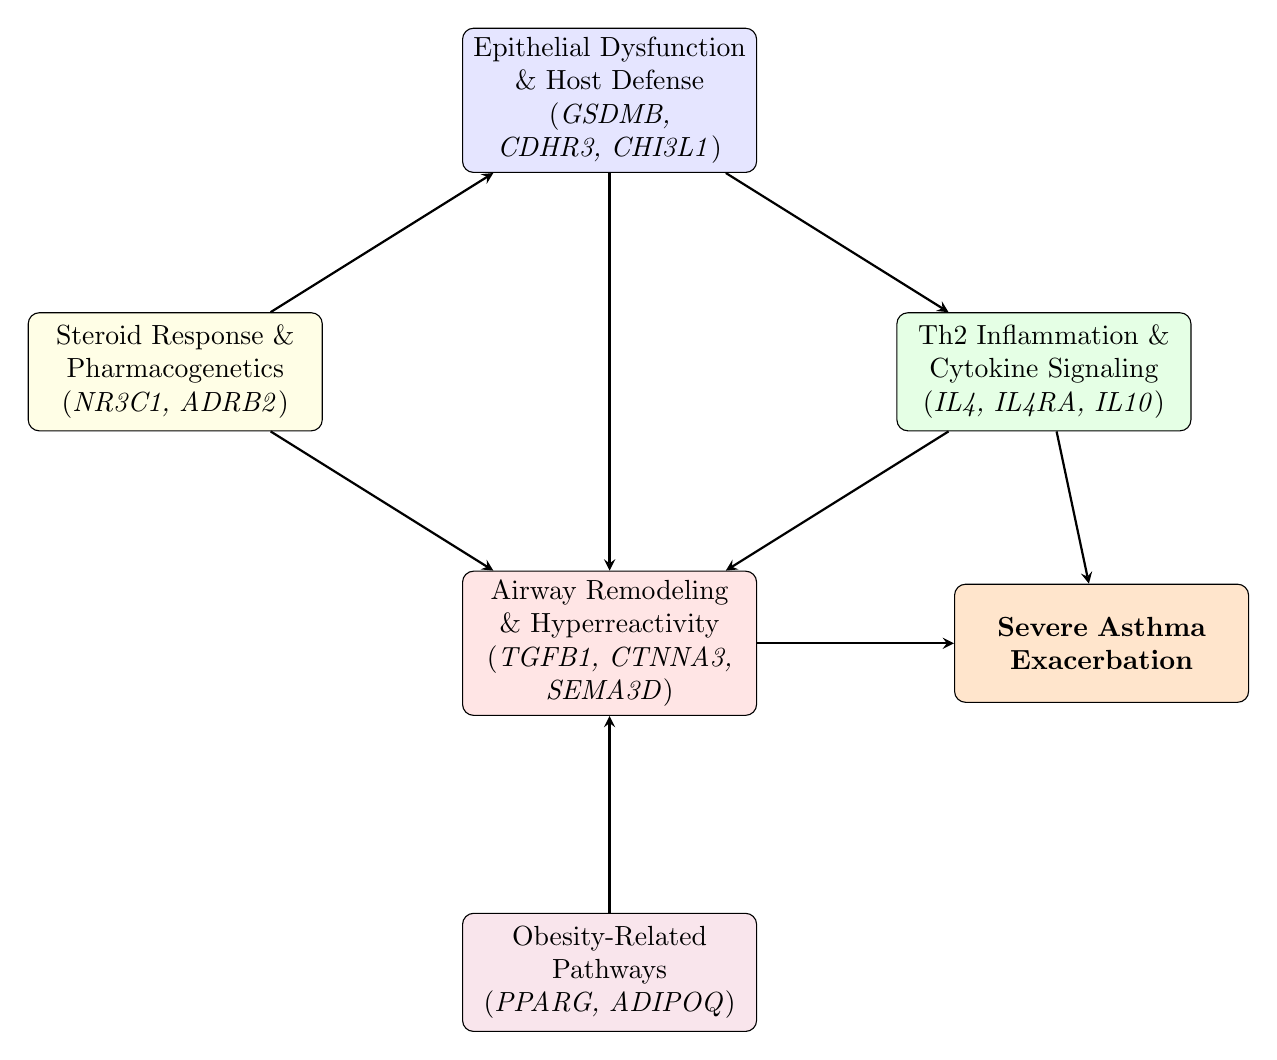
\begin{tikzpicture}[
    node distance=2.5cm,
    box/.style={rectangle, draw, rounded corners, text width=3.5cm, align=center, minimum height=1.5cm},
    arrow/.style={thick,->,>=stealth}
]

% Nodes
\node (epithelial) [box, fill=blue!10] {Epithelial Dysfunction \& Host Defense \\ (\textit{GSDMB, CDHR3, CHI3L1})};
\node (th2) [box, fill=green!10, below right=of epithelial] {Th2 Inflammation \& Cytokine Signaling \\ (\textit{IL4, IL4RA, IL10})};
\node (steroid) [box, fill=yellow!10, below left=of epithelial] {Steroid Response \& Pharmacogenetics \\ (\textit{NR3C1, ADRB2})};
\node (remodeling) [box, fill=red!10, below right=of steroid] {Airway Remodeling \& Hyperreactivity \\ (\textit{TGFB1, CTNNA3, SEMA3D})};
\node (obesity) [box, fill=purple!10, below=of remodeling] {Obesity-Related Pathways \\ (\textit{PPARG, ADIPOQ})};
\node (exacerbation) [box, fill=orange!20, right=of remodeling] {\textbf{Severe Asthma Exacerbation}};

% Arrows
\draw [arrow] (epithelial) -- (th2);
\draw [arrow] (epithelial) -- (remodeling);
\draw [arrow] (th2) -- (remodeling);
\draw [arrow] (steroid) -- (remodeling);
\draw [arrow] (steroid) -- (epithelial);
\draw [arrow] (obesity) -- (remodeling);
\draw [arrow] (th2) -- (exacerbation);
\draw [arrow] (remodeling) -- (exacerbation);

\end{tikzpicture}
\caption{Genetic Architecture of Asthma Exacerbation Susceptibility}
\label{fig:bio_model}
\end{figure}

\clearpage

\subsection*{Supplementary Tables}

\noindent\textbf{Supplementary Table S1: Full Search Strategy}
\begin{longtable}{@{}p{2.5cm}p{12.5cm}@{}}
\toprule
\textbf{Database} & \textbf{Search Query} \\
\midrule
\endfirsthead
\midrule
\textbf{Database} & \textbf{Search Query} \\
\midrule
\endhead
\bottomrule
\endfoot
\bottomrule
\endlastfoot
PubMed & ("Asthma"[Mesh] OR "asthma"[Title/Abstract]) AND ("Asthma/complications"[Mesh] OR "Disease Progression"[Mesh] OR "Exacerbation*"[Title/Abstract] OR "Severe"[Title/Abstract] OR "Hospitalization"[Title/Abstract]) AND ("Polymorphism, Single Nucleotide"[Mesh] OR "Polymorphism"[Title/Abstract] OR "SNP"[Title/Abstract] OR "Variant"[Title/Abstract] OR "Genome-Wide Association Study"[Mesh] OR "GWAS"[Title/Abstract]) AND (ADRB2 OR IL4 OR IL4RA OR TNFA OR NR3C1 OR PPARG OR TGFB1 OR IL10 OR CHI3L1 OR GSDMB OR CTNNA3 OR ADIPOQ OR SEMA3D) \\
\midrule
Embase & ('asthma'/exp OR asthma:ti,ab) AND ('disease exacerbation'/exp OR exacerbation:ti,ab OR severe:ti,ab OR hospitalization:ti,ab) AND ('single nucleotide polymorphism'/exp OR SNP:ti,ab OR variant:ti,ab OR GWAS:ti,ab) AND (ADRB2 OR IL4 OR IL4RA OR TNFA OR NR3C1 OR PPARG OR TGFB1 OR IL10 OR CHI3L1 OR GSDMB OR CTNNA3 OR ADIPOQ OR SEMA3D) \\
\midrule
GWAS Catalog & (Asthma) AND (Exacerbation) \\
\midrule
Search Limits & English language, Human subjects, Inception to January 2023 \\
\end{longtable}

\noindent\textbf{Supplementary Table S2: Characteristics of Key Included Studies} \\
\textit{Note: Only a representative subset of the 45 included studies is displayed for brevity.}
\begin{longtable}{@{}p{3.5cm}p{2cm}p{3cm}p{2.5cm}p{3.5cm}@{}}
\toprule
\textbf{Study / Cohort} & \textbf{Design} & \textbf{Population} & \textbf{Genes} & \textbf{Main Finding} \\
\midrule
\endfirsthead
\midrule
\textbf{Study / Cohort} & \textbf{Design} & \textbf{Population} & \textbf{Genes} & \textbf{Main Finding} \\
\midrule
\endhead
\bottomrule
\endfoot
\bottomrule
\endlastfoot
CAMP \& CARE \cite{McGeachieWu2015} & GWAS & Pediatric (North America) & \textit{CTNNA3, SEMA3D} & rs7915695 significantly associated with high exacerbation rates. \\
COPSAC \cite{ParkTantisira2017} & Cohort & Pediatric Birth Cohort (Denmark) & \textit{GSDMB, CDHR3} & \textit{GSDMB} rs7216389 increased hazard of hospitalizations. \\
PiCA Consortium \cite{FarzanVijverberg2018} & Meta-analysis & Multi-ancestry Pediatric & \textit{GSDMB} & rs7216389 associated with hospitalizations despite ICS. \\
UK Biobank \cite{FawcettHall2025} & GWAS & Adult (UK) & \textit{ADRB2} & rs1042713 not associated in adults. \\
SARP \cite{LiChristenson2021} & Cohort & Pediatric/Adult Severe Asthma & \textit{GSDMB, ORMDL3} & rs2305480 linked to longitudinal exacerbations. \\
BREATHE, GALA II \cite{TurnerFrancis2016} & Meta-analysis & Pediatric & \textit{ADRB2} & \textit{ADRB2} Arg16 increased AE risk with LABA. \\
BioVU \cite{McGeachieWu2015} & EHR Cohort & Multi-ancestry (USA) & \textit{SEMA3D} & \textit{SEMA3D} risk specific to African American cohort. \\
PACMAN \cite{DijkVijverberg2019} & Cohort & Pediatric & \textit{IL1RL1} & rs13431828 associated with ED visits. \\
\end{longtable}

\noindent\textbf{Supplementary Table S3: Risk-of-Bias Assessment (Newcastle-Ottawa Scale for Key Studies)}
\begin{longtable}{@{}lcccc@{}}
\toprule
\textbf{Study} & \textbf{Selection (0-4)} & \textbf{Comparability (0-2)} & \textbf{Outcome (0-3)} & \textbf{Total (0-9)} \\
\midrule
\endfirsthead
\midrule
\endhead
\bottomrule
\endfoot
\bottomrule
\endlastfoot
McGeachie et al. (CAMP/CARE) \cite{McGeachieWu2015} & 4 & 2 & 3 & 9 (Low Risk) \\
Park et al. (COPSAC) \cite{ParkTantisira2017} & 4 & 2 & 3 & 9 (Low Risk) \\
Farzan et al. (PiCA) \cite{FarzanVijverberg2018} & 4 & 2 & 2 & 8 (Low Risk) \\
Turner et al. \cite{TurnerFrancis2016} & 4 & 2 & 2 & 8 (Low Risk) \\
Sood et al. \cite{SoodConnolly2018} (EHR) & 3 & 1 & 2 & 6 (Moderate Risk) \\
Li et al. (SARP) \cite{LiChristenson2021} & 4 & 2 & 3 & 9 (Low Risk) \\
\end{longtable}

\noindent\textbf{Supplementary Table S4: GRADE Summary of Findings for Key Loci}
\begin{longtable}{@{}lp{2cm}p{2cm}p{2cm}p{2cm}p{2cm}p{1.5cm}@{}}
\toprule
\textbf{Gene/SNP} & \textbf{Risk of Bias} & \textbf{Inconsistency} & \textbf{Indirectness} & \textbf{Imprecision} & \textbf{Publication Bias} & \textbf{Overall Quality} \\
\midrule
\endfirsthead
\midrule
\endhead
\bottomrule
\endfoot
\bottomrule
\endlastfoot
\textit{GSDMB} rs7216389 & Not serious & Not serious & Not serious & Not serious & Undetected & \textbf{High} \\
\textit{CDHR3} rs6967330 & Not serious & Not serious & Not serious & Not serious & Undetected & \textbf{High} \\
\textit{ADRB2} rs1042713 & Not serious & Serious & Not serious & Not serious & Undetected & \textbf{Moderate} \\
\textit{IL4RA} rs1801275 & Not serious & Serious & Not serious & Not serious & Undetected & \textbf{Moderate} \\
\textit{TGFB1} rs1800469 & Serious & Serious & Not serious & Serious & Undetected & \textbf{Very Low} \\
\textit{SEMA3D} rs993312 & Not serious & Serious & Not serious & Serious & Undetected & \textbf{Low} \\
\end{longtable}

\bibliographystyle{unsrt}
\bibliography{references}

\end{document}
